\documentclass[tikz]{standalone}

\usepackage{circuitikz}
\usepackage{siunitx}

\begin{document}
	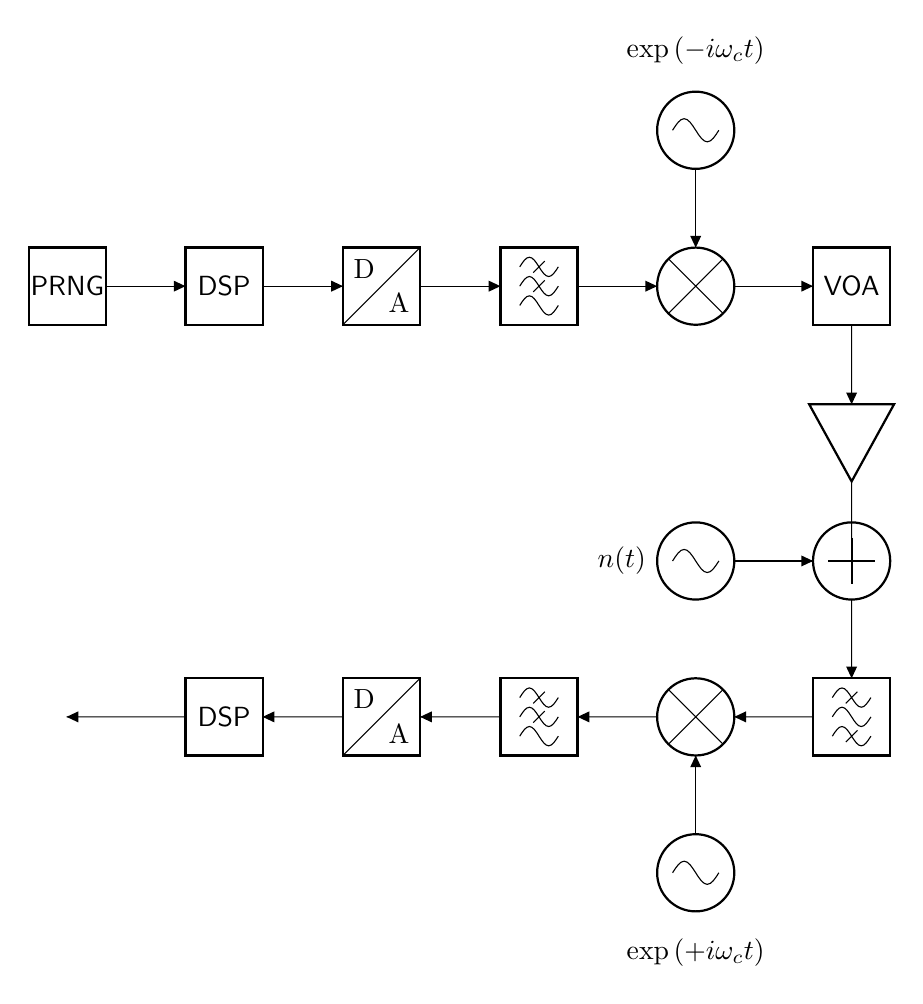
\begin{tikzpicture}
		\draw (0,0) node[twoportshape, t=\textsf{PRNG}, anchor=east](prng){} to[dsp, >] ++(3,0)
			to[dac,>] ++(1,0)
			to[lowpass, >] ++(3,0)
			node[inputarrow]{}
			node[mixer, anchor=west](mixer){};
		\draw (mixer.north) node[inputarrow, rotate=-90]{} to[short] ++(0,1) node[oscillator, anchor=south]{} ++(0,1.5) node{$\exp\left(-i\omega_ct\right)$};
		\draw (mixer.east) to[short] ++(1,0) node[inputarrow]{} node[twoportshape, t=\textsf{VOA}, anchor=west](voa){};
		\draw (voa.south) to[amp, >] ++(0,-3) node[adder](adder){};
		\draw (adder.west) node[inputarrow]{} to[short] ++(-1,0) node[oscillator]{} ++(-1,0) node[left]{$n(t)$};
		\draw (adder.south) to[short] ++(0,-1) node[inputarrow, rotate=-90]{} node[bandpassshape, anchor=north](bp){};
		\draw (bp.west) to[short] ++(-1,0) node[inputarrow, rotate=180]{} node[mixer, anchor=east](mixer2){};
		\draw (mixer2.south) node[inputarrow, rotate=90]{} to[short] ++(0,-1) node[oscillator, anchor=north]{} ++(0,-1.5) node{$\exp\left(+i\omega_ct\right)$};
		\draw (mixer2.west) to[lowpass, >] ++(-3,0)
							to[adc, >] ++(-1,0)
							to[dsp, >] ++(-3,0)
							to[short] ++(-0.5,0) node[inputarrow, rotate=180]{};
	\end{tikzpicture}
\end{document}
